%************************************************
\chapter{Introduction}\label{ch_intro}
%************************************************

Over the past decade, the comparative analysis of genomic sequences
has immeasurably expanded our understanding of the evoluion, biology
and diversity of mammals, the taxonomic class to which we belong
%\citep{Lander2001,Mouse2002Initial,Rat2004Genome,LindbladToh2005Genome,
%  Sequencing2005a,Margulies2007}.
Although the revolution in genomic
medicine that was optimistically predicted during the unveiling of the
draft human genome sequence is still far from being realized
\citep{Collins2001,Varmus2010}, the impact of comparative genomics on
the study of human evolution, diversity and biology has been more
immediate, far-reaching and deep \citep{OBrien1999,Lander2011}. Many
important questions in evolution have been asked---for example, what
is the rate of mammalian speciation
\citep{BinindaEmonds2007,Venditti2011}, or what is the fraction of the
genome under functional constraint
\citep{Boffelli2003a,Siepel2005,Ponting2011}---and, to some extent
answered, using large amounts of genomic data.

The aim of this thesis is to show how the large-scale comparative
analysis of genes and genomes can be used to identify genomic regions
and biological features which have been subject to exceptional levels
of selective constraint throughout mammalian evolution. When shared
across many species, these evolutionary patterns can highlight genes
and pathways involved in ongoing, universal mammalian genetic
conflicts \citep{CastilloDavis2004}; when observed in one or a few
lineages, they may indicate more specific adaptations related to those
species' unique evolutionary hsitory \citep{Sawyer2005a,Nielsen2007}.

Furthermore, along with the increased use of high-throughput methods
and datasets in biology has come a heightened awareness of the
inescapable presence of noise and error within data. The study of
genome sequences is no exception to this point; indeed, the many
potential sources of error in any comparative genomic analysis combine
to make it difficult to assess accuracy or to identify anomalous
results. This is especially problematic in comparative genomic
analyses, where genome sequencing and sequence alignment errors can be
mistaken for interesting biological signals
\citep{Mallick2009,Schneider2009,Fletcher2010,MarkovaRaina2011}. Some
of the difficulty of assessing results stems from a limited
understanding of how various sources of error can impact downstream
evolutionary analyses; thus, a secondary aim of this thesis is to
better understand the impact of error on large-scale comparative
analyses, and to further develop methods for appropriately predicting
and handling such error.

\section{The evolution of mammals and the mammalian genome}

A major motivating factor behind the sequencing and study of mammalian
genomes has been the desire to shed light on the human genome sequence
through comparative study, leading to a better understanding of the
diversity of genomic constraints under which our species has evolved
\citep{Mouse2002Initial}. As the genome sequence of every animal is
intertwined with all aspects of its biology, any comparison of genomes
must be performed within the context of each species' phenotypic
traits and evolutionary history; it will thus be useful to briefly
review some salient features of the evolutionary history of mammals
and their genomes which will serve as useful background for the
analyses presented in this thesis.

Mammals are a diverse class of vertebrates, comprising roughly 5,400
species whose common ancestor lived ca. 165--170 \ac{myr} ago
\citep{Wilson2005}. According to a comprehensive supertree constructed
by Bininda-Emonds et al. using a combination of molecular data and
fossil calibrations, the earliest major branching events were the
split of Monotremata (containing the egg-laying mammals such as
platypus and echidna) around 166 \ac{myr} ago and the divergence of
the Marsupialia and Placentialia orders around 150 \ac{myr} ago. By
100 \ac{myr} ago the major placental superorders (e.g., Afrotheria,
Euarchontoglires, Laurasiatheria and Xenarthra) had all diverged, and
nearly all extant mammalian orders originated prior to 85 \ac{myr} ago
\citep{BinindaEmonds2007}. These dates were somewhat earlier than what
had commonly been estimated based purely on fossil evidence
\citep{Archibald2001}, but the early mammalian fossil record is
sparse, which lends weight to the argument that the true date of
origin is several \ac{myr} before the earliest discovered
fossil. Taking this effect into account, an independent statistical
analysis of primate fossils provided corroborating evidence for the
relatively early divergence of mammalian lineages
\citep{Martin2007}. The Bininda-Emonds et al. phylogeny suggests that
43 placental lineages with extant descendants survived through the
mass extinction at the K/T boundary, during which up to two-thirds of
all mammalian species went extinct \citep{Alroy1999}. After a 10
\ac{myr} period of overall decreased diversification levels
(e.g. lowered speciation rates), most mammalian lineages continued to
diversify at a relatively constant rate
\citep{BinindaEmonds2007,Martin2007}.

This evolutionary history has influenced the shape of the phylogenetic
tree relating the extant mammalian species, a summarized version of
which is shown in Figure \ref{fig_mammals_10k}. (Note that the dates
of some of the earliest branches of the phylogeny in Figure
\ref{fig_mammals_10k}, which was adapted from \citet{Haussler2009}
using data from \citet{Hedges2009}, disagree with the above
description based on \citet{BinindaEmonds2007}, reflecting the large
amount of uncertainty regarding more ancient events.) Deep but
relatively short branches separate most of the ordinal groups, with
the exception of Marsiupialia and Monotremata, which are separated
from the other mammalian orders by much longer distances. Within each
order, a fairly regular pattern of branching is seen (note, however
that the tree in Figure \ref{fig_mammals_10k} is truncated at the
family level, omitting the relationships of individual species). Most
orders are represented by several extant species, suggesting that the
branch length separating any one species from its closest relative is
fairly small, again with the exception of Monotremata which contains
only 5 species spanning 45 \ac{myr}. These aspects of the mammalian
phylogeny make it well-suited for large-scale comparative analysis, as
long branches separating sequenced genomes (which are a major source
of alignment error and uncertainty in evolutionary reconstruction) can
continue to be shortened by sequencing additional species. Indeed,
this was part of the motivation behind the \ac{mgp}
\citep{LindbladToh2011}, which generated much of the data used
throughout this thesis and which I will introduce in more detail in
Chapter \ref{ch_orthologs}.

\begin{figure}
\centering
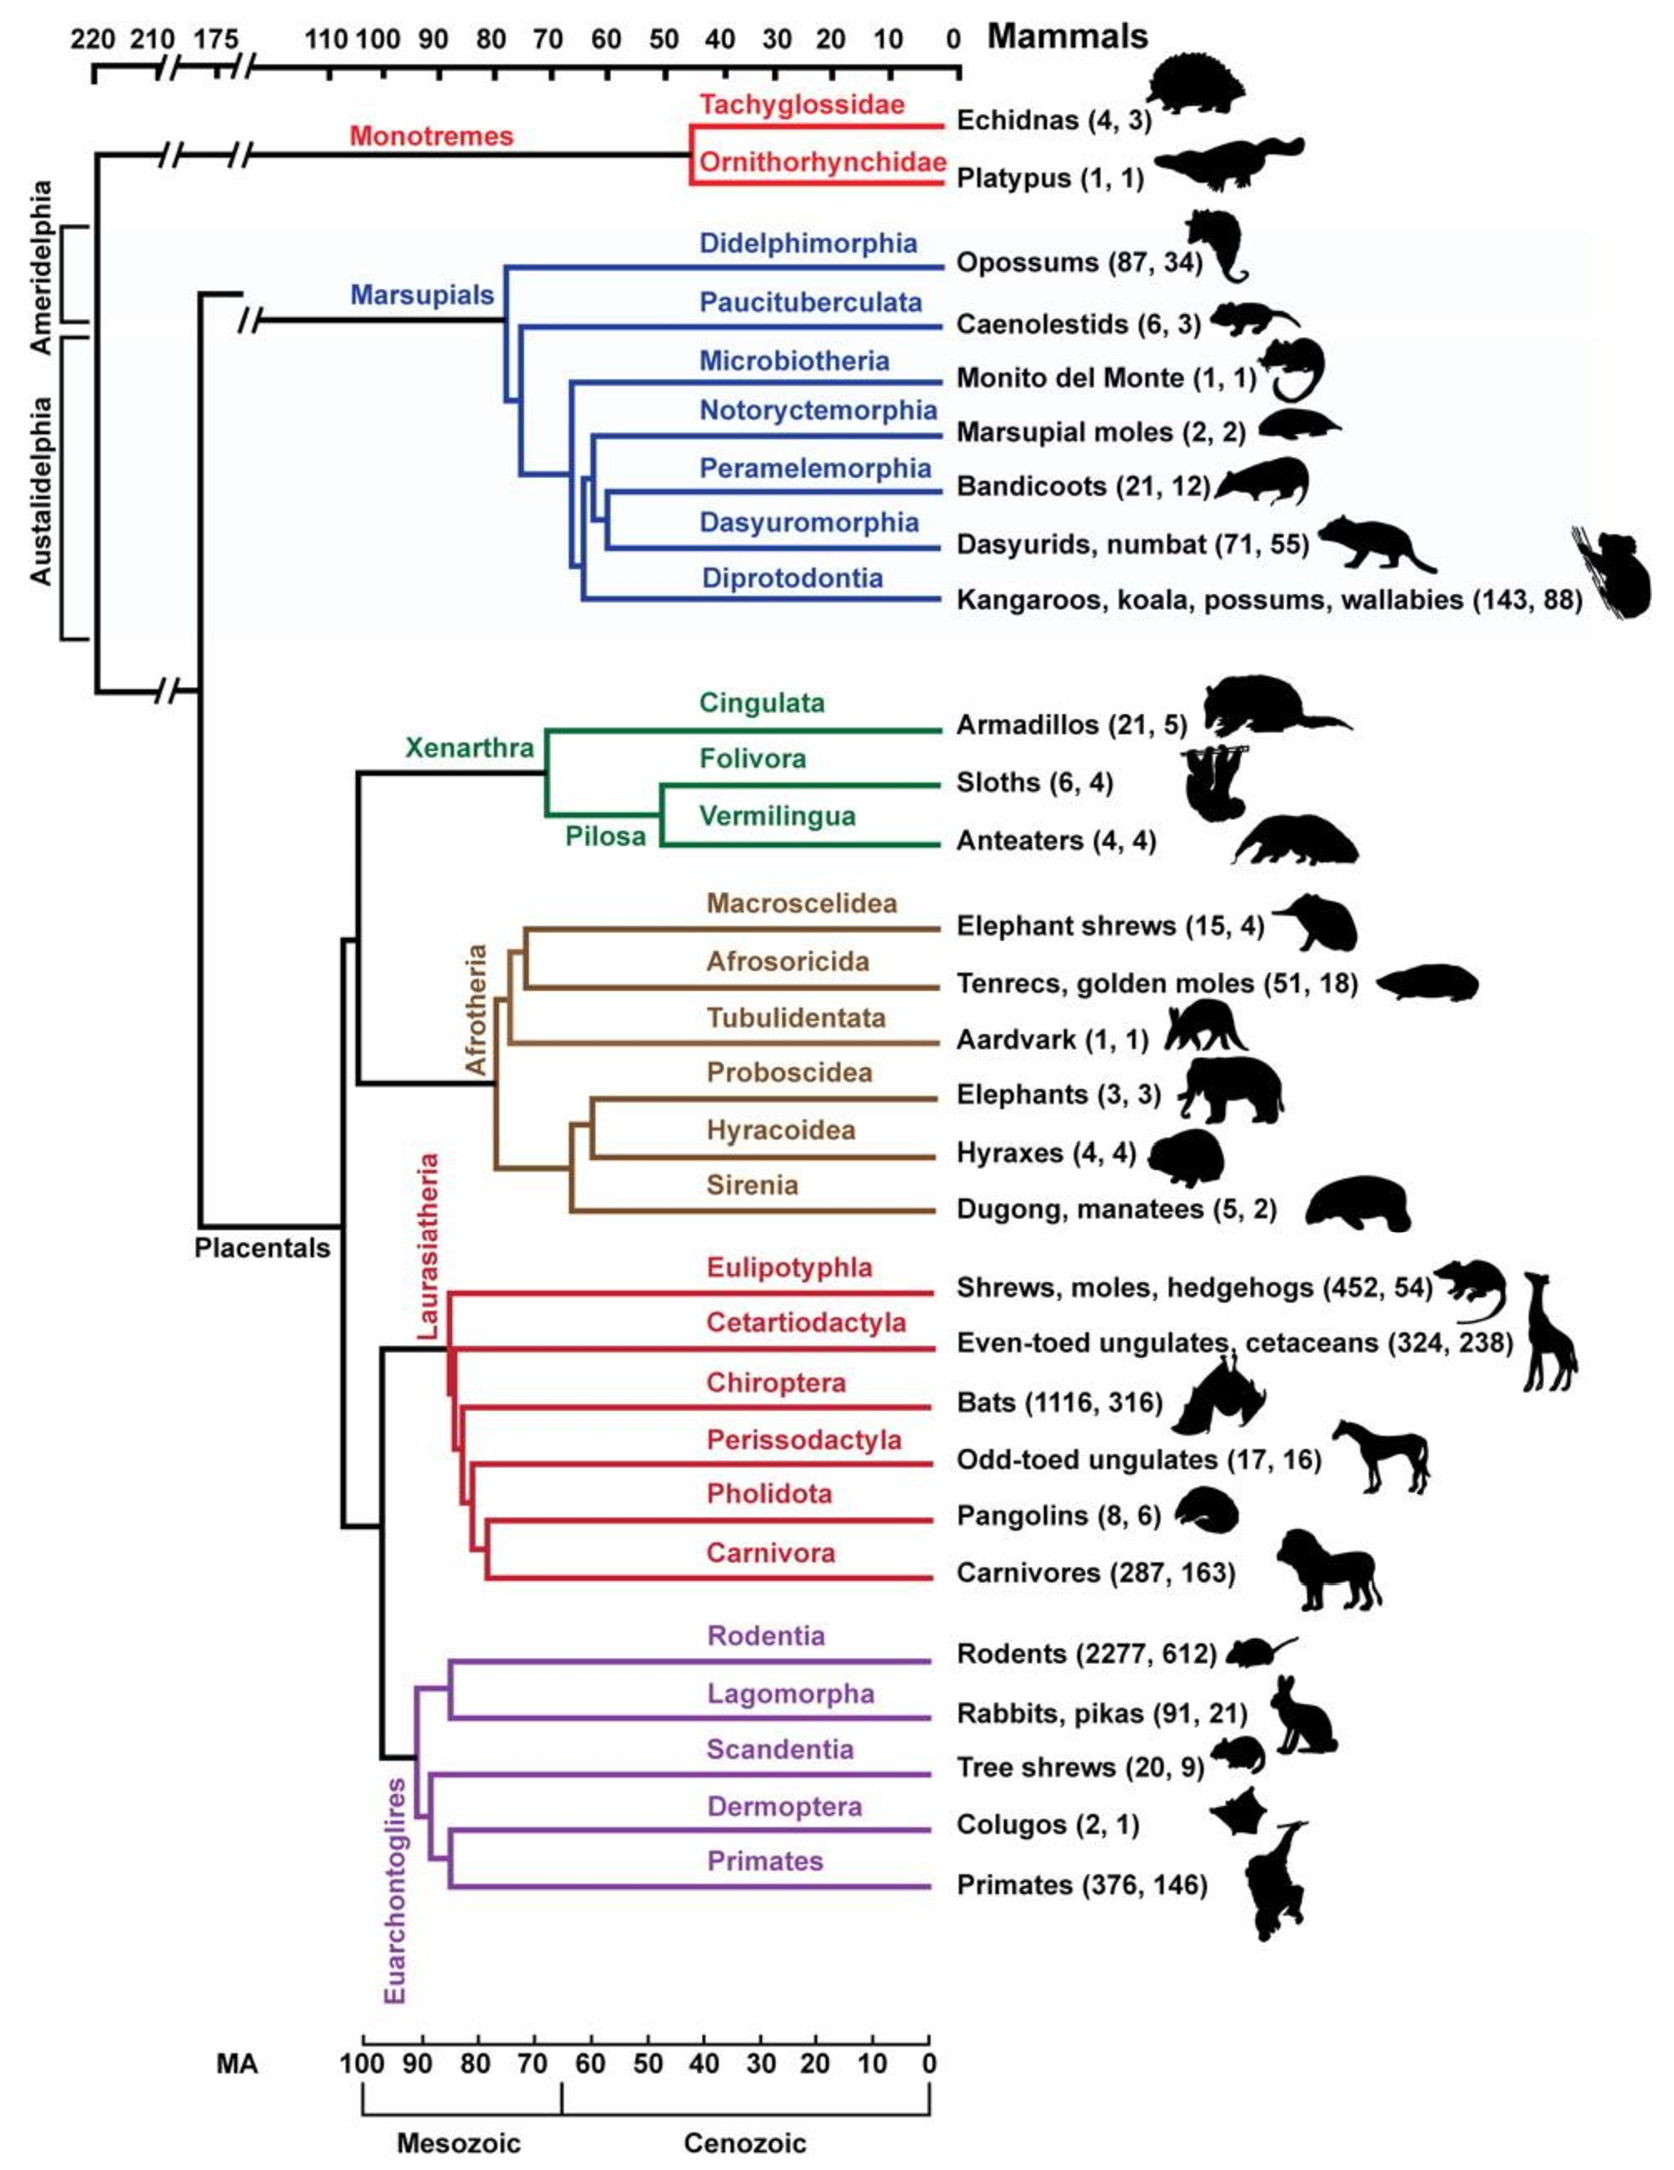
\includegraphics[scale=0.5]{Figs/mammals_10k.pdf}
\caption{A time-resolved consensus phylogeny of the major mammalian
  lineages. Topologies and dates use data from Hedges and Kumar
  \citeyearpar{Hedges2009}. Each terminal branch represents a
  mammalian family. The number of species contained in each family is
  included as the first number in parentheses after each family name
  (e.g., there are 2,227 species of rodents). Figure taken from
  \citet{Haussler2009}. }
\label{fig_mammals_10k}
\end{figure}

Before the K/T boundary, ancestral mammal and primate species were
likely smaller in size than they are today, as the ecological niches
for larger animals were occupied by dinosaurs
\citep{Martin2008,Smith2010}. Their diet is assumed to have been
largely insectivorous, as folivory in extant species is observed
mainly in larger mammals \citep{Smith2010} (but see \citet{Martin2007}
for an alternative perspective favoring a more folivorous primate
ancestor). After the K/T extinction event around 65 \ac{myr} ago,
mammals eventually diversified to occupy a wide range of the
ecological roles left vacant by extinct species, with many lineages
undergoing highly specialized morphological and behavioral adaptations
and the range of mammalian body sizes expanding by four orders of
magnitude \citep{Alroy1998}. A long-term trend towards larger body
sizes has been observed in many lineages; the hypothesis that this is
a general feature of mammalian evolution has been termed Cope's rule
\citep{Alroy1998}, though its universality is controversial
\citep{Finarelli2006,Monroe2010}.

The body size of mammals and their ancestors is an important
consideration in sequence analyses, as body size has been shown to
correlate with the overall rate of substitution in multicellular
eukaryotes
\citep{Mouse2002Initial,Hwang2004a,Welch2008,Galtier2009,Romiguier2010,
  Bromham2011}.  Other phenotypic features, such as metabolic rate and
generation time, have been similarly linked to genomic evolutionary
rates \citep{Martin1993,Nabholz2008}, but all three of these
characters are strongly cross-correlated in mammals, making it
difficult to isolate the effect of each particular variable on the
overall evolutionary rate or to identify the causative factor behind
such variation. Regardless, it is clear that extant mammals exhibit a
wide range of neutral evolutionary rates \citep{BinindaEmonds2007b},
with proposed explanatory factors including differences in the amount
of mutagenic free radicals associated with an animal's metabolic rate,
different rates of germ line cell divisions per year, and different
DNA repair control mechanisms \citep{Baer2007}.

\begin{figure}
\centering
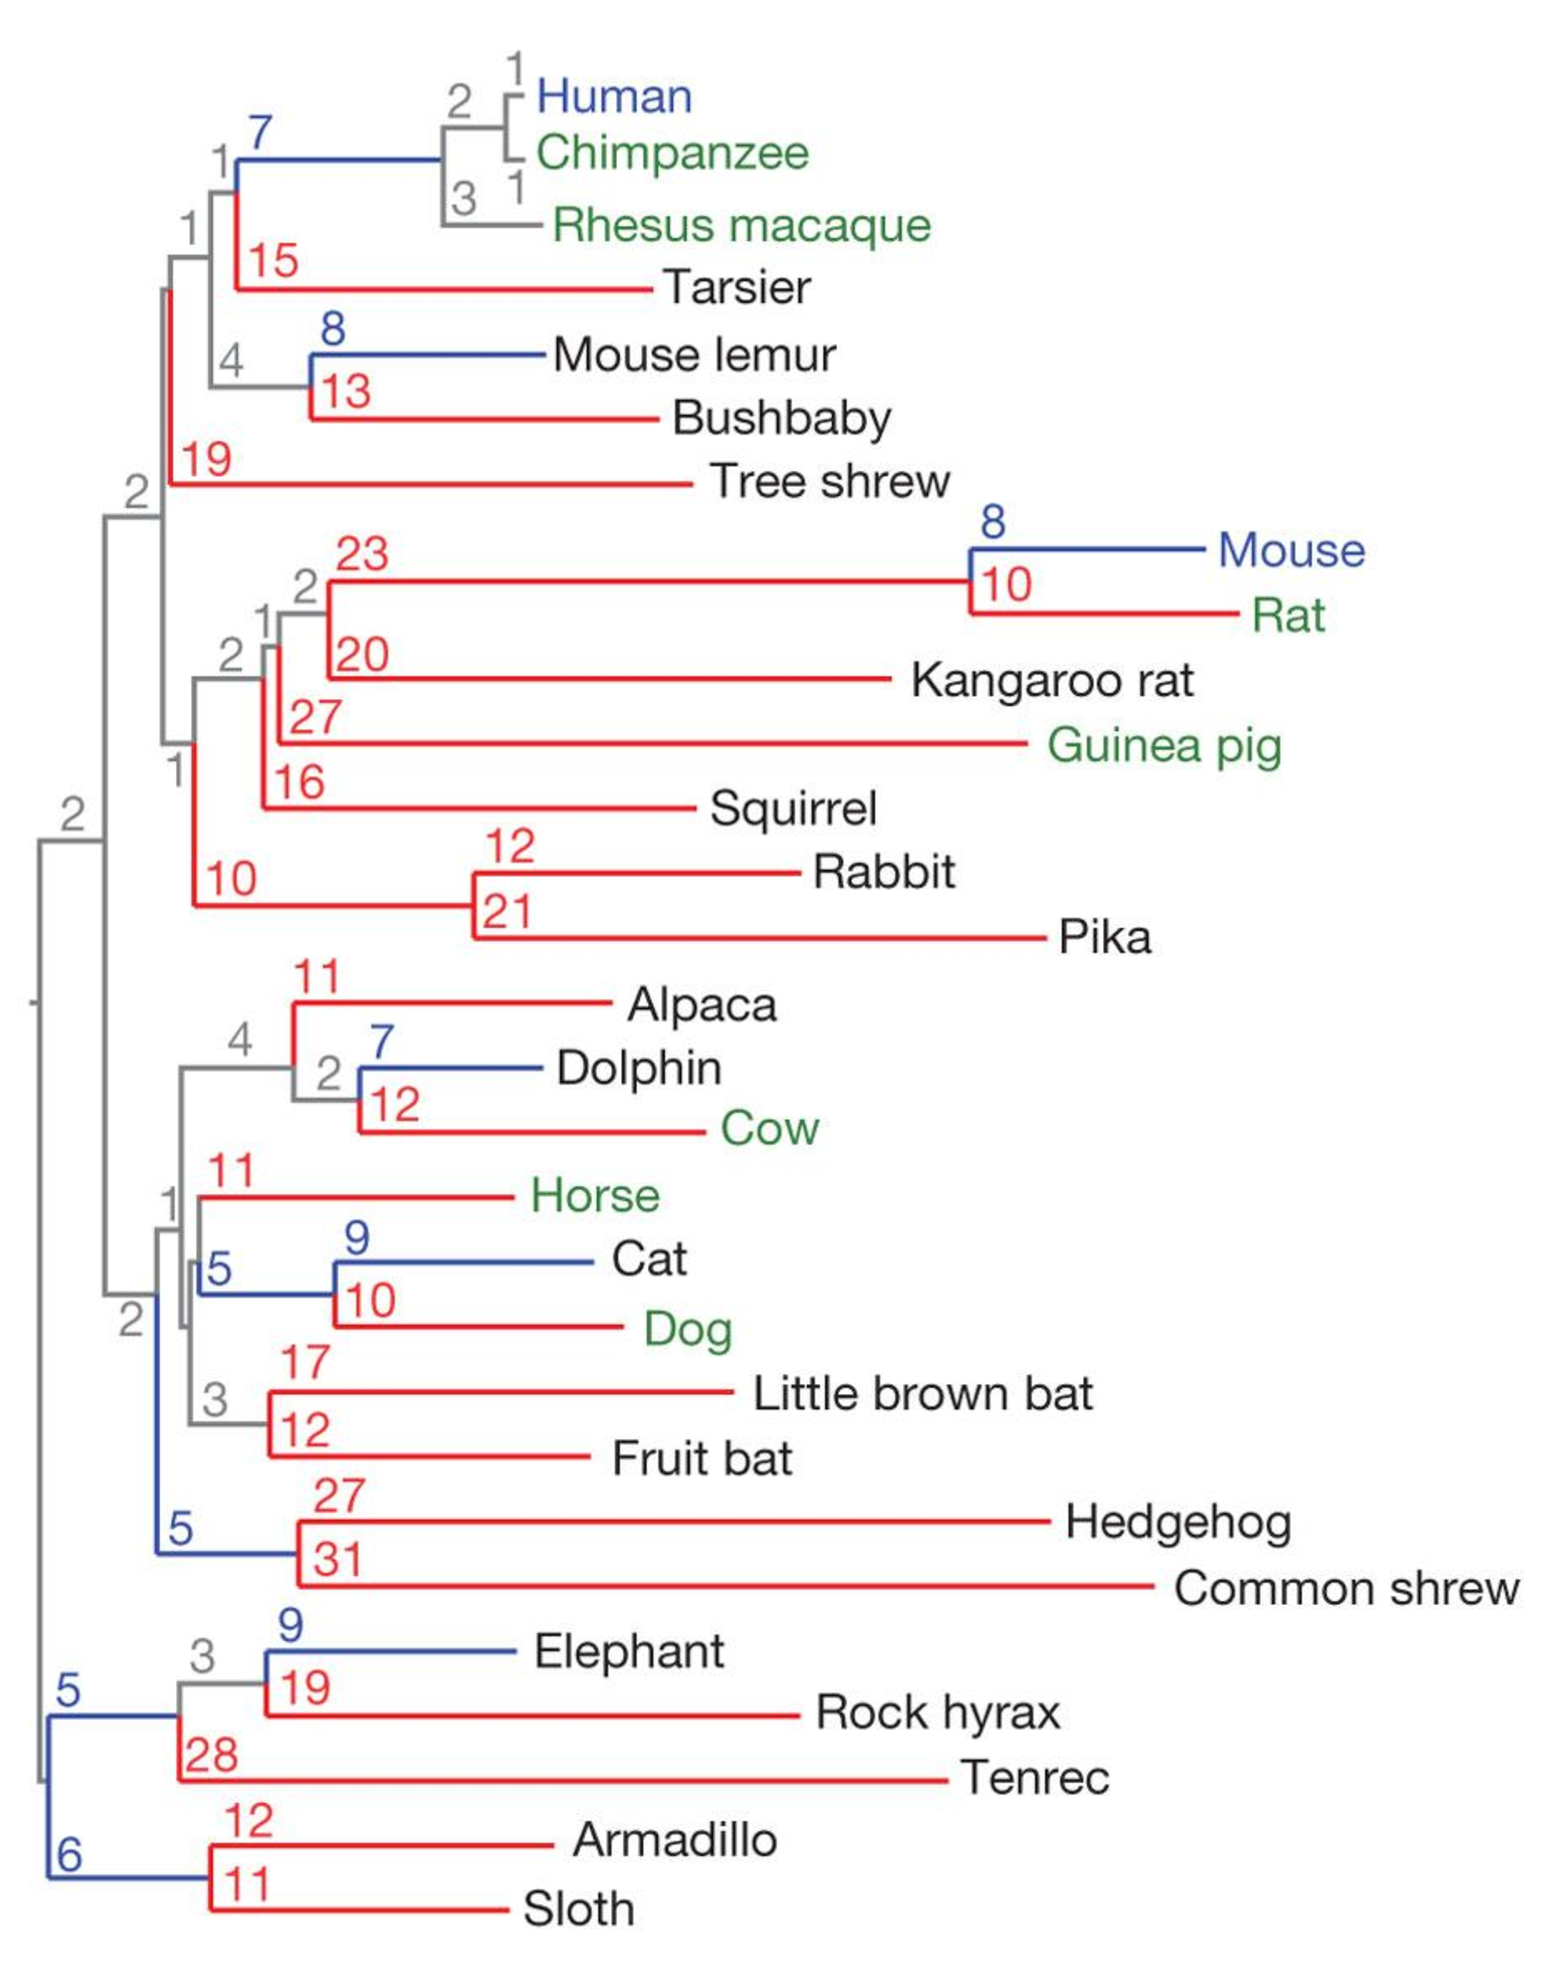
\includegraphics[scale=0.3]{Figs/mammals_29.pdf}
\caption{A phylogeny of 29 mammalian species, with branch lengths
  scaled with the neutral evolutionary rate estimated from genome-wide
  DNA alignments. Note the increased branch lengths of most rodent
  species (e.g., mouse, rat, pika) and various small members of
  Laurasiatheria (e.g., little brown bat, hedgehog, common shrew)
  relative to most primates (e.g., human, chimpanzee). Figure taken
  from \citet{LindbladToh2011}.}
\label{fig_mammals_29}
\end{figure}

The correlation between body size and neutral evolutionary rate has an
important consequence for comparative genomic studies in mammals:
extant species groups with smaller body sizes are expected to have
experienced more DNA substitutions since their common ancestor than
larger-bodied species groups, leading to increased branch lengths
within smaller-bodied clades when branches are scaled by the neutral
evolutionary rate. Figure \ref{fig_mammals_29} shows a phylogenetic
tree for 29 mammals scaled by the genome-wide rate of observed
substitutions, emphasizing the high observed substitution rates of
most rodents and low rates of most hominids and some larger-bodied
species from other mammalian orders. In comparative analyses where a
larger number of substitutions increases the power of a method to
detect a genomic feature or estimate an evolutionary rate (e.g., in
detecting conserved regulatory elements or positive selection), the
larger branch lengths of rodent species would be expected to result in
improved power and statistical accuracy. This effect will be
especially important in Chapter~\ref{ch_mammals1}, where I compare \sw
estimates of selection pressures from groups of species from different
mammalian orders.

A second biological characteristic showing significant variation
between mammals, the \ac{ne}, has important consequences for the study
of genomic regions subject to natural selection
\citep{Charlesworth2009}. \ac{ne} is a fundamental parameter in
population genetics, describing the size of an idealized population
that exhibits the same amount of dispersion of allele frequencies due
to genetic drift as the real population under study
\citep{Wright1931,Woolfit2009}. Many aspects of a population can
influence its \ac{ne}, including the census count, breeding patterns,
and geographical distribution of individuals \citep{Caballero1994},
and studies within mammals have consistently shown a much larger
\ac{ne} for rodents than for primates and for small versus large
mammals \citep{EyreWalker2002,Popadin2007,Halligan2010}, suggesting
that extant mammalian populations can significantly vary in this
parameter. It is beyond the scope of this thesis to provide a
comprehensive discussion of \ac{ne} and its importance within
population genetics and molecular evolution, but \citet{Woolfit2009}
and \citet{Charlesworth2009} provide focused reviews of the
subject. The main predicted impact of \ac{ne} on the study of fixed
substitutions between species is that slightly deleterious mutations
are more likely to become fixed within a population having a small
\ac{ne} versus a population with a large \ac{ne}. Closely tied to this
effect is the prediction of the nearly neutral thoery of molecular
evolution \citep{Kimura1985} that many mutations in protein-coding
regions are slightly deleterious and thus subject to this dependence
on \ac{ne} \citep{Kimura1974a,Kimura1985,Ohta1992}. Several empirical
studies have supported this hypothesis, showing that a different
\ac{ne} leads to different rates of protein evolution in bacteria
\citep{Moran2008,Warnecke2011}, birds \citep{Axelsson2009} and mammals
\citep{Kosiol2008,Ellegren2009} (but see \citet{Bachtrog2008} for
potentially contradictory evidence from \emph{Drosophila}). Any
analysis of comparative evolution in mammals should thus evaluated
with respect to these well-established trends; in Chapters~
\ref{ch_mammals1} and~\ref{ch_mammals2} I consider the possible
effects of \ac{ne} on the observed patterns of positive selection
within different groups of mammals, and in Chapter~\ref{ch_gorilla} I
use genome-wide comparisons to estimate ancestral \ac{ne} in our
closest primate relatives.

Key features of the mammalian genome itself are also worth
highlighting. Mammals contain relatively large genomes (roughly 3 Gb
of DNA, ranging from 2.5 to 4.5 Gb) with between 20 to 80 chromosomes
\citep{Bachmann1972}. The large range in chromosome count is likely a
result of the high rate of chromosomal rearrangement in mammals
\citep{Eichler2003,Pevzner2003}. Some regions of ``rearrangement
hotspots'' show especially large amounts of large-scale genomic
shuffling within mammals, and it has been speculated that these
regions have contributed to the many lineage-specific gene family
expansions in mammals \citep{Eichler2003}. Breakpoints of mammalian
chromosomal rearrangements tend to occur near transposable elements
\citep{Zhao2009}, which are small DNA sequences capable of replicating
throughout the genome \citep{Lander2001}. Transposable elements, a
diverse class of sequence elements representing a variety of
transposition mechanisms and sequence characteristics, together
comprise roughly 45\% of DNA in the human genome and have contributed
signifciantly the ancient and ongoing evolution of mammalian genomes
\citep{Lander2001,Cordaux2009}.

In contrast to the rapid turnover of noncoding DNA and high rate of
genomic rearrangement observed in mammalian genomes, the
protein-coding gene complement appears to be less variable. Initial
estimates of roughly 30,000 protein-coding
\citep{Lander2001,Mouse2002Initial} genes in the human and mouse
genomes have been lowered based on accumulating functional and
phylogenetic evidence to roughly 21,000 genes \citep{Macaque2007}; the
most recent gene annotations from \ens \citep{Flicek2011} contain
20,599 human and 21,873 mouse protein-coding genes. A majority of
these genes are shared between all mammals'' human and mouse are
estimated to share 80\% of genes in a ``one-to-one'' fashion, meaning
no apparent gene duplications or deletions occurred since the common
ancestor \citep{Mouse2002Initial}, and a wider group of mammals
including platypus show detectable orthologs (including genes with
duplications or deletions in one or more lineages) in 82\% of genes
\citep{Warren2008b}. Despite the relative consistency of the mammalian
protein-coding catalogue, features such as alternative splicing and
domain concatenations have been identified as potential contributors
to mammalian phenotypic complexity and diversity \citep{Lander2001}.

In any study of vertebrate protein-coding genes, the \ac{2r}
hypothesis looms large. Originally proposed by \citet{Ohno1970}, the
\ac{2r} hypothesis suggests that two polyplidization events occurred
during the early evolution of the vertebrate common ancestor,
explaining the observation that vertebrates often have up to four
homologs of invertebrate genes \citep{Hokamp2003}. For three decades
the veracity of the \ac{2r} hypothesis was hotly debated
\citep{McLysaght2002,Dehal2005}, but analyses based on comparisons
between whole-genome sequences of several fish and basal chordates
have repeatedly confirmed its predictions
\citep{Kasahara2007,Putnam2008b}. In addition to having interesting
implications for the evolution of the immune system and of
morphological diversity within vertebrates
\citep{Hughes1997,Hoffmann1999,Peer2009b} the existence of ancient
genomic duplications can cause problems in the inference of homology
relationships between genes. Many of these aspects will be considered
in more detail in Chapter~\ref{ch_orthologs} when a set of mammalian
orthologs suitable for evolutionary analysis is identified.

\section{Models of sequence evolution}
\label{codon_intro}

The above section described several important genomic and evolutionary
features of the mammalian clade. Many of those well-established
observations resulted from the application of mathematical models of
sequence evolution to comparative genomics data, which is now a
widespread analytical appraoch. This section briefly introduces a
selection of important methods and models for evolutionary analysis
which will be applied throughout the remaining chapters.

As the hereditary material of all free-living organisms, DNA
represents a record of the history of life on earth. When an
individual gives rise to offspring, some segments of DNA are
replicated and passed on to all its descendants; importantly, the
processes of DNA replication and repair are imperfect
\citep{Arnheim2009}, and the resulting errors---called mutations---are
passed on to successive generations. In addition to being a major
source of the variation between individuals invoked in Darwin's theory
of natural selection \citep{Darwin1859a}, mutations in DNA leave a
molecular record of evolutionary relationships and of the passage of
time. The gradual accumulation of mutations in DNA, commonly observed
as differences in DNA sequences between species at the same homologous
location, can be reasonably modeled using phylogenetic trees and
Markov models of sequence change \citep{Yang2006}.

The earliest observations that biological sequences tend to randomly
change over time were made from the sequences of proteins, which are
cellular molecules comprised of amino acid units whose arrangement is
encoded in the DNA sequences of exons within genes. Zuckerkandl and
Pauling, who were analyzing the amino acid sequences of hemoglobin
genes from various species, noted in 1962 that the number of changes
between sequences from different species corresponded well with the
evolutionary distance those species based on fossil evidence; this led
them to hypothesize that evolution at a molecular level may occur at a
largely constant rate \citep{Zuckerkandl1962,Morgan1998}. Zuckerkandl
and Pauling continued to explore the implications and applications of
their ``molecular evolutionary clock'' hypothesis, using hemoglobin
and cytochrome C sequences, for example, to estimate the date of
human-gorilla divergence (at 11 million years) and to infer the
ancestral protein sequences of mammalian ancestors
\citep{Zuckerkandl1965}. Since those pioneering studies in proteins, a
variety of evolutionary models have been developed to describe
observed patterns of amino acid and DNA substitution. As this thesis
is concerned largely with the application of such methods, I will only
briefly summarize the key features of the more popular evolutionary
models; \citet{Yang2006} provides a comprehensive mathematical
treatment.

The simplest model of DNA substitution, proposed by
\citet{Jukes1969a}, assumes that every nucleotide has the same rate of
changing into any other nucleotide. Although the assumption of equal
rates may be reasonable for modeling a random process, the point
mutation of a DNA base pair is a biochemical process (or rather, a set
of potentially many unobserved biochemical processes which all produce
the same class of observable result) which may contain biases towards
or against certain types of mutations. This was quickly discovered to
be the case: analysis of the ever-increasing number of available
biological DNA sequences showed that in many datasets
\emph{transitions}, defined as substitutions between two pyrimidine
nucleotides (e.g., T$\to$C or C$\to$T) or between two purine
nucleotides (e.g., A$\to$G or G$\to$A), are more common than
\emph{transversions}, defined as substitutions from a purine to a
pyrimidine or vice-versa. \citet{Kimura1980} thus proposed a more
complex model, called K80 or Kimura's two-parameter model, which
accounted for this bias. Specifically, Kimura's K80 model extends JC69
by incorporating an additional parameter, $\kappa$, referred to as the
transition/transversion ratio, which represents the ratio of the rate
of transition versus the rate of transversion substitutions. When
$\kappa$ is greater than one, transitions occur at a higher rate than
transversions, providing a better fit to most biological datasets. The
$\kappa$ parameter of K80 a prototypical example of the parametric
approach to building evolutionary models, where a parameter is
introduced into the model which allows for a commonly-violated
assumption of the simpler model to be relaxed. The value of the
parameter is not specified in the model, however; it is usually
estimated from the data on a case-by-case basis from the data using
\ac{ml} \citep{Whelan2001}.

Several nucleotide models were subsequently described which relax
various assumptions of the JC69 and K80 models
\citet{Whelan2001,Yang2006}. One especially unrealistic feature of K80
is its symmetric nature (meaning that the rate of substitution from
one nucleotide to another is the same as the rate of the reverse
substitution, e.g. G$\to$C = C$\to$G). A symmetric DNA Markov chain
yields equal nucleotide frequencies when the substitution process
reaches equilibrium, meaning that any starting DNA sequence, if left
to evolve long enough under such a process, will end up with equal
nucleotide frequencies. In reality, many biological sequences contain
highly unequal nucleotide frequencies (owing to a variety of possible
selective or mutationsal biases), making it inappropriate to assume an
equal base composition \citep{Yang2006}. Thus, models such as FEL
\citep{Felsenstein1981a}, HKY \citep{Hasegawa1985} and TN93
\citep{Tamura1993} were developed to allow for various combinations of
unequal base frequencies and an unequal transition/transversion
ratio. The most general reversible nucleotide model, REV
\citep{Tavare1986}, includes four parameters describing the
equilibrium nucleotide frequencies and six rate parameters, one for
each possible pair of substitutions.

In contrast to the primarily parametric DNA models, evolution models
for amino acid substitutions have generally been estimated empirically
\citep{Whelan2001}. Developed during the early days of evolutionary
sequence analysis, the JTT \citep{Jones1992} and Dayhoff
\citep{Dayhoff1978} amino acid models were estimated using
parsimony-based counting methods. The parsimony principle was first
used to infer phylogenetic trees and ancestral protein sequences from
each set of aligned proteins within a large database. Based on those
phylogenetic trees and ancestral sequences, the entries of the 20x20
amino acid substitution matrix were populated with counts of inferred
amino acid substitutions, and these counts were used to estimate a
Markov substitution model. More recently, empirical amino acid models
were estimated using \ac{ml} methods, which improved upon a number of
methodological issues with the parsimony approach
\citep{Adachi1996,Whelan2001b}.

A few important assumptions are shared by all of the models already
described, namely that all sites within an alignment are (a) evolving
independently of one another, (b) evolving under the same evolutionary
process and at the same evolutionary rate (c) related by the same
underlying phylogenetic tree. I will briefly review the development of
models which relax these assumptions, all of which are clearly
violated in many real datasets.

Independence between sites is generally a difficult assumption to
relax for computational reasons \citep{TODO}, but the hypermutability
of CpG dinucleotides within mammalian genomes (where CpG denotes a C
nucleotide followed by a G nucleotide, the ``p'' representing the
phosphodiester bond separating nucleotides on the same strand of a DNA
molecule) has provided strong impetus to incorporate at least a
dinucleotide context into models for estimating nucleotide
substitution rates from large mammalian alignments
\citep{Blake1992,Hwang2004a,Siepel2004a}. CpG hypermutability results
from the methylation and subsequent deamination of the cytosine
nucleotide at CpG sites in most mammalian genomic DNA; although all
cytosine nucleotides are prone to deamination, cytosine deamination
produces uracil, which is removed by uracil glycosylase allowing for
DNA repair mechanisms to replace the original cytosine, while
5-methylcytosine produces thymidine, which results in frequent C$\to$T
transitions \citep{Ehrlich1982,Hwang2004a}. Context-dependent
substitution models have shown that CpG mutations are by far the
dominant form of mutation in mammalian genomes, and such models have
also been essential for studying the evolution of GC content and
mammalian isochores \citep{Duret2006,Duret2008}.

The major violation of the assumption of the same evolutionary rate
and model between sites is the observation that the

  \draft{Introduce the idea of modeling protein evolution as a markov
    process acting on codon sequences: the incorporation of
    mechanistic parameters for Ts:Tv bias (kappa), dN/dS ratio
    (omega), or empirical models a la . Talk about heterogeneity
    the idea that real data may strongly violate certain models.}

\section{Detecting purifying and positive selection in proteins}
\label{pos-sel_intro}

  \draft{Briefly run through the history of detecting purifying /
    positive selection in genes and sites. Mention history of PAML
    models, alternative approaches, and fully describe SLR's
    approach.}

  \draft{SLR implements a method specifically designed for sitewise
    estimates which has been shown in sim- ulations to perform as well
    as or better than PAML’s sitewise random sites models (Massingham
    and Goldman, 2005). SLR models codon evolution as a
    continuous-time Markov process where substitutions at one site are
    independent of substitutions at all other sites. No assumptions
    are made regarding the distribution of ω ratios within the
    alignment. The value of ω is considered to be an independent
    parame- ter at each site: after first optimizing shared parameters
    using the whole alignment, SLR uses the shared parameters and the
    data at each alignment site to calculate a sitewise statistic for
    non-neutral evolution.  This statistic is based on a
    likelihood-ratio test where the null model is neutral evolution (ω
    = 1) and the alternative model is either purifying or positive
    selection (ω < 1 or ω > 1, respectively). The raw statistic
    measures the strength of evidence for non-neutral evolution at
    each site; following Massingham and Goldman (2005) we use a signed
    version of the SLR statistic (created by negating the statistic
    for sites with ω < 1) as the test statistic for positive
    selection.}


\section{Outline of the thesis}

In this thesis, I describe... three studies concerning the use of
phylogenetic codon models to identify

